%File: paper.tex — AAAI 2026 Submission
\documentclass[letterpaper]{article}
\usepackage[submission]{aaai2026}
\usepackage{times}
\usepackage{helvet}
\usepackage{courier}
\usepackage[hyphens]{url}
\usepackage{graphicx}
\urlstyle{rm}
\def\UrlFont{\rm}
\usepackage{natbib}
\usepackage{caption}
\frenchspacing
\setlength{\pdfpagewidth}{8.5in}
\setlength{\pdfpageheight}{11in}
\usepackage{amsmath}
\usepackage{booktabs}
\usepackage{multirow}

% Search for figures: figures/ subfolder first, then analysis/figures
\graphicspath{{./}{figures/}{figures/instruction_effect/}{figures/agreement_variants/}{figures/agreement_heatmaps/}{figures/agreement_scatter/}{figures/accuracy_quadrant/}{figures/confidence_dist/}{figures/scale_plots/}{figures/entity_analysis/}{../../../analysis/figures/}{../../../analysis/figures/agreements/}}

% TODO markers for placeholder content
\newcommand{\TODO}[1]{\textbf{[TODO: #1]}}
\newcommand{\PLH}[1]{\textit{[Placeholder: #1]}}

% Placeholder figure box (remove when real figure is ready)
\newcommand{\figplaceholder}[2]{%
  \fbox{\parbox{#1}{\centering\vspace{0.8cm}\small\textit{#2}\vspace{0.8cm}}}%
}

\pdfinfo{
/TemplateVersion (2026.1)
}

\setcounter{secnumdepth}{2}

\title{When Models Answer Without Seeing: Human-Calibrated Diagnosis\\
of Linguistic Prior Exploitation in Vision-Language Models}

\author{Anonymous}
\affiliations{Anonymous Institution}

\begin{document}

\maketitle

% ─────────────────────────────────────────────────────────────────────────────
\begin{abstract}
Analogous to hypothesis-only baselines that exposed annotation artifacts in
Natural Language Inference \citep{poliak2018hypothesis}, we investigate how
much of VQA behavior is explainable without any visual information.
Across multiple open-source Vision-Language Models (VLMs), blind inference
reveals characteristic answer distribution biases shaped by the training
distribution \citep{mccoy2024embers}: models collapse to ``no'' for yes/no
questions and ``0'' for count questions at rates far exceeding human baselines.
To characterize how these priors depend on lexical cues, we introduce
\emph{control question variants}: four progressively weaker reformulations that
remove entity anchors while preserving question type. A single instruction
further reveals a spectrum from \emph{instruction-gated} prior use to
unconditional hallucination. Blind outputs are also highly overconfident:
their token-confidence distributions remain high even for wrong committed
answers, a calibration failure
invisible to accuracy-only evaluations. Using a human blind-answer dataset
(N=36, 113 questions, IRB-approved), we show that the model group closest to
human blind priors is not the full VLM but the VLM backbone decoder: removing
the vision encoder yields the highest human-model semantic agreement, while
full VLMs and standalone LLMs exhibit distinct failure regimes. Question-type
analysis then reveals where this overlap comes from: yes/no and action
questions show strong human-model prior sharing, while count and
grounded-reference questions are strongly anti-aligned.
\end{abstract}

% ─────────────────────────────────────────────────────────────────────────────
\section{Introduction}

Vision-Language Models (VLMs) achieve impressive performance on visual question
answering (VQA) benchmarks \citep{antol2015vqa,goyal2016making}, yet a basic
question remains unanswered: how much of this performance reflects genuine
visual grounding, and how much can be explained by linguistic priors inherited
from large-scale language model pretraining?

This question parallels a well-known episode in Natural Language Inference
(NLI): \citet{poliak2018hypothesis} showed that a model trained on hypotheses
alone---ignoring the corresponding premises---substantially exceeded the random
baseline across ten NLI datasets. The finding revealed annotation artifacts
embedded in the benchmarks themselves. We apply the same diagnostic logic to
VQA: the \emph{image} plays the role of the premise, and the question is the
hypothesis. A model that answers correctly from the question alone is exploiting
a hypothesis-only shortcut.

\citet{mccoy2024embers} provide the mechanistic explanation: large language
models are shaped by their training objective over internet-scale text, and
therefore produce outputs proportional to the probability of sequences in the
training corpus. When a VQA question has a high-frequency answer in training
data (``What color is the sky?'' $\to$ ``blue''), a VLM will produce that answer
reliably regardless of the image. Blind VQA accuracy thus directly measures
corpus frequency exploitation.

In this work, we conduct a diagnostic study of this phenomenon across multiple
open-source VLMs. The paper is organized around three questions.
First, how much blind accuracy can models obtain at scale, and what answer
distribution biases underlie that performance?
Second, how does prior-driven behavior change when we remove lexical anchors or
explicitly instruct the model to answer from a plausible imagined scene?
Third, how similar are blind model behaviors to human blind reasoning at the
levels of correctness, answer distribution, and semantic agreement?

To answer these questions, we combine blind evaluation on 1,000 VQA questions,
a control-variant perturbation suite, token-confidence analysis from output
logprobs, and a
human blind-answer dataset (N=36 participants, 113 questions). The goal is not
to claim that blind answering is inherently illegitimate; the goal is to
identify \emph{which} priors are shared with humans and \emph{which} are
model-specific artifacts---a distinction that prior accuracy-centric diagnostics
cannot make.

\paragraph{Main findings.}
\begin{enumerate}
    \item Models answer a substantial fraction of VQA questions correctly
    without any image input, confirming that blind prior exploitation is
    pervasive rather than anecdotal.

    \item VLM backbone decoders (language backbone without the vision encoder)
    are the model group most closely aligned with human blind priors. They
    reach the highest human-model semantic agreement, while full VLMs are lower
    and standalone LLMs diverge further.

    \item Full VLMs and standalone LLMs do not simply share a generic ``model
    prior.'' They exhibit different failure regimes: full VLMs show stronger
    no-bias and zero-bias, while standalone LLMs are more heterogeneous and
    often less human-aligned in answer semantics.

    \item Models exhibit characteristic null-hypothesis biases under blind
    conditions: 62\% of VLM yes/no answers are ``no'' (vs.\ human 33\%),
    70\% of count answers are ``0'' (vs.\ human 5\%), and color answers cluster
    on ``black''. These biases are model-specific---not shared with
    human blind reasoners.

    \item Human-model prior alignment then explains where this split comes
    from: yes/no and action questions show strong overlap, while count and
    grounded-reference questions are anti-aligned. This identifies which
    priors are genuinely human-like and which are model-specific artifacts.

    \item Blind outputs are severely overconfident: wrong committed answers
    remain in a high-confidence regime, and the instruction further raises
    confidence while reducing abstention, indicating more committed
    hallucination rather than more grounded reasoning.
\end{enumerate}

\paragraph{Methodological contributions.}
Beyond the empirical findings, this work introduces two reusable diagnostic tools.

\textbf{(i) A semantic control-question extraction pipeline.} For each VQA
question, we use GPT-4.1-mini with a structured JSON schema to automatically
generate four progressively weaker reformulations: deictic markers removed,
object noun replaced by a neutral placeholder, object replaced by its one-level-up
hypernym, and content nouns fully pronominalized. This forms a controlled
degradation axis that isolates \emph{which lexical elements} carry prior information,
independently of accuracy. The pipeline is fully specified (prompt and schema in
Appendix~\ref{app:ctl}) and applicable to any VQA benchmark.

\textbf{(ii) An operation--entity taxonomy for VQA prior analysis.} We annotate
each question with a semantic \emph{operation type} (yes/no-existence, count,
attribute, action, world knowledge, spatial, identity, temporal, text/OCR,
comparison, causal) and an \emph{entity type} (person, animal, object, food,
vehicle, place, etc.). This taxonomy enables fine-grained diagnosis: yes/no and
action questions show near-perfect human--model prior alignment (Jaccard
$\approx 0.93$), while count and OCR questions are anti-aligned
($r = -0.39$)---a distinction invisible at the aggregate level.
Together, the two tools provide a principled diagnostic vocabulary for studying
linguistic prior exploitation in any multimodal benchmark.

% ─────────────────────────────────────────────────────────────────────────────
\section{Related Work}

\paragraph{Hypothesis-Only and Shortcut Baselines.}
\citet{poliak2018hypothesis} demonstrated that NLI classifiers achieve
non-trivial accuracy using only the hypothesis, exposing annotation artifacts.
\citet{gururangan2018annotation} further characterized these artifacts through
systematic analysis of annotation bias. In VQA, \citet{agrawal2018dont} showed
that models relying on question-answer co-occurrence statistics could achieve
high accuracy without visual understanding. Our work extends this diagnostic
tradition by providing a human reference dataset alongside model evaluations,
enabling calibrated measurement of the gap.

\paragraph{LMs as Corpus Frequency Models.}
\citet{mccoy2024embers} showed that LLM failure patterns are predicted by three
factors: the probability of the task, the input, and the output in the training
corpus. Models are biased toward high-probability outputs regardless of task
requirements. We operationalize this insight: blind VQA accuracy directly
measures the probability of question-answer pairs in the pretraining distribution.

\paragraph{VLM Hallucination and Shortcut Learning.}
Hallucination in VLMs---confident generation of visually ungrounded
content---has been widely documented \citep{ji2023survey,rohrbach2018object,
xiao2021hallucination}. \citet{chen2024are} proposed MMStar to audit visual grounding by filtering
out questions solvable without images. VLind-bench
\citep{lee2024vlind} specifically measures language prior influence across
diverse benchmarks. \citet{han2024instinctive} identified visual shortcuts
through spurious image features. Complementarily, \citet{kim2025subtlebench}
show that VLMs fail at fine-grained visual discrimination even when images are
present---together with our work, bounding the visual grounding gap from both
directions: models answer without images when they should not, and fail to
use images when they must.

\paragraph{Human Cognition Under Uncertainty.}
Human reasoning under missing information is well characterized by dual-process
theory \citep{tversky1974judgment,kahneman2011thinking}: fast, heuristic
System~1 thinking relies on representativeness and availability, while System~2
engages deliberate reasoning when cues are insufficient. Studying how humans
answer questions without visual evidence thus belongs to a well-established
research tradition in psycholinguistics and cognitive modeling---examining what
mechanisms govern speculation under uncertainty \citep{bar2007proactive}.
Critically, humans do not share the corpus-frequency bias of pretrained LLMs:
their yes-bias (67\% ``yes'') reflects pragmatic plausibility rather than
training-distribution statistics, making human blind behavior the natural
reference for what \emph{linguistically natural} uncertainty looks like.

% ─────────────────────────────────────────────────────────────────────────────
\section{Experimental Setup}

\subsection{Models and Datasets}
\label{sec:setup}

We evaluate open-source VLMs from the Qwen3-VL \citep{bai2025qwen3vl} and LLaVA
\citep{liu2023visual,liu2024llavanext} families, plus Qwen3
\citep{yang2025qwen3} LLMs as text-only baselines. The main blind-performance
table reports the model subset for which the current zero-shot results are
fully assembled; additional instruction-only comparisons are reported
separately in Appendix~\ref{app:inst}. All models are evaluated in zero-shot
settings with temperature 0.

Our primary evaluation dataset consists of 1,000 questions sampled from the
VQA v2.0 validation split \citep{goyal2016making}, spanning yes/no,
numerical, and open-ended question types. For the human alignment analysis
(Section~\ref{sec:alignment}), we use the 113-question subset
on which the human study was conducted.

\subsection{Blind Inference Conditions}

We evaluate models under three conditions: (1) \textbf{Standard}: the original
image with the question; (2) \textbf{Blind}: a blank 224$\times$224 white PNG
replacing the original image; and (3) \textbf{Blind+Inst}: blank image with an
additional instruction appended to the question: ``\textit{Note: No images are
provided. For each question, imagine an appropriate image exists and answer
based on the most common or universal scenario.}''

\subsection{Control Question Variants and Semantic Taxonomy}
\label{sec:control}

As a methodological contribution, we introduce two annotation layers applied to
all 1{,}000 VQA questions.

\textbf{Control question extraction.}
To characterize \emph{how} models exploit linguistic priors, we generate four
progressively weaker reformulations of each question using
GPT-4.1-mini (temperature 0, seed 42, JSON schema mode) for reproducibility:

\begin{enumerate}
    \item \textbf{deictic\_removed}: Deictic markers (\textit{this, that, here,
    there}) and spatial qualifiers (left/right/top/bottom) are removed while
    preserving fluency. Tests whether spatial anchoring drives shortcut behavior.

    \item \textbf{object\_removed}: The specific object noun is replaced with the
    neutral placeholder ``object.'' Tests the contribution of entity identity to
    prior exploitation.

    \item \textbf{weaker\_object}: The specific noun is replaced with a
    one-level-up hypernym (dog $\to$ animal, car $\to$ vehicle, shirt $\to$
    clothing). Tests whether category-level identity is sufficient to trigger
    prior recall.

    \item \textbf{pronominalized}: All content noun phrases are replaced with
    minimal pronouns following grammar-aware rules (``What color is the dog?''
    $\to$ ``What color is it?''; ``How many cats are there?'' $\to$ ``How many
    are there?''). This maximally removes entity-specific prior cues while
    preserving question structure.
\end{enumerate}

The degradation chain from original $\to$ \texttt{pronominalized} forms a
monotonically decreasing axis of lexical prior cues, enabling a controlled
measurement of how much each entity reference contributes to shortcut
exploitation. The GPT extraction prompt and JSON schema are provided in
Appendix~\ref{app:ctl}.

\textbf{Operation--entity taxonomy.}
Each question is also annotated by the same GPT pipeline with two semantic
dimensions: (1)~\emph{operation type}---the question's cognitive demand:
yes/no-existence (\texttt{exist}), counting (\texttt{count}), attribute
identification (\texttt{attr}), action recognition (\texttt{act}), world
knowledge (\texttt{know}), spatial reasoning (\texttt{spat}), object
identification (\texttt{ident}), temporal reasoning (\texttt{temp}),
text/OCR (\texttt{text}), comparison (\texttt{comp}), and causal reasoning
(\texttt{cause}); and (2)~\emph{entity type}---the primary visual referent:
person, animal, object, food, vehicle, place, and other.
These two dimensions cross-classify the 1{,}000 questions and enable the
fine-grained alignment analysis in Section~\ref{sec:prior_types}, where we show
that human--model prior alignment varies dramatically across operation types
(Jaccard $0.93$ for yes/no vs.\ $0.13$ for count), a distinction invisible at
the aggregate level and unreachable without the taxonomy.

\subsection{Human Data Collection}

We recruited N=36 participants (15 men, 21 women; age 18--34) through online
university community forums. All procedures were conducted under an
IRB-approved protocol (compensation: 10,000 KRW/hour, consistent with
standard rates). Participants answered 113 VQA-style questions in a text-only
blind setting, relying only on the question text and general world knowledge.
Responses could be given in Korean or English and were translated and normalized
prior to analysis. After each answer, participants rated their confidence on a
5-point Likert scale. Unless otherwise noted, the human-comparison analyses in
Section~\ref{sec:alignment} are matched to the model condition used for those
exports rather than assumed to be interchangeable across all blind prompts.
Full protocol details are provided in Appendix~\ref{app:human}.

\subsection{Metrics}

We use four metric families, with different roles in the paper.

\textbf{Task accuracy.}
We report \textbf{VQA accuracy} using the standard 10-annotator soft evaluation
\citep{antol2015vqa}. This serves as context for how much blind success models
obtain, but it is not our primary evidence for human-like prior structure.
At the question level, human accuracy $h(q)$ is the proportion of 36
participants judged correct on question $q$; model accuracy is binary at the
single-answer level.

\textbf{Answer-distribution overlap.}
To measure whether humans and models converge on the same blind answers even
when they are not always correct, we compute \textbf{Jaccard overlap of the
top-3 answers} per question. For human answer set $H_q$ and model answer set
$M_q$, this is:
\[
\mathrm{Jaccard}(q) = \frac{|H_q \cap M_q|}{|H_q \cup M_q|}.
\]
This metric captures shared prior structure independently of exact correctness.

\textbf{Agreement and semantic similarity.}
For the answer-agreement analyses in Section~\ref{sec:alignment}, we compare
human-human, human-model, and model-model answer pairs after shared answer
normalization. We use two classes of agreement metrics.

First, \textbf{lexical metrics}: \textbf{exact match}, \textbf{token Jaccard},
\textbf{ROUGE-1}, and \textbf{chrF}. These quantify increasingly soft surface
overlap, from exact normalized identity to word- and character-level overlap.

Second, \textbf{semantic metrics}: \textbf{Sentence-BERT cosine}
\citep{wang2020minilm}, \textbf{SimCSE cosine}, and \textbf{BERTScore F1}.
These are the main metrics for our central claim, because the question is not
whether models reproduce the exact human string, but whether they recover the
same human prior at the level of meaning. In the main text, Sentence-BERT is
the primary semantic metric; the others are used as robustness checks.

\textbf{Alignment and reliability.}
To compare human and model difficulty patterns across questions, we compute
\textbf{Pearson difficulty correlation}, namely Pearson $r$ between per-question
human accuracy $h(q)$ and per-model accuracy. We prefer Pearson over rank-based
alternatives because the comparison is over proportions and the relationship is
approximately linear in the current analyses. To quantify group consistency, we
also report \textbf{Krippendorff's $\alpha$} (nominal scale) for within-group
and cross-group inter-rater reliability.

\textbf{Confidence.}
Finally, we measure a \textbf{token-confidence proxy} from generation
logprobs (top-5 token logprobs, temperature 0). For each answer, we convert
each generated token logprob to probability and average across generated
tokens. This produces a mean token probability in $[0,1]$, which we use to
characterize whether blind answers are cautious, abstaining, or confidently
hallucinated.

% ─────────────────────────────────────────────────────────────────────────────
\section{Linguistic Prior Exploitation: Distribution Biases and Prior Structure}
\label{sec:prior}

We characterize the \emph{structure} of blind model behavior---what answer
distributions models produce, and how those distributions depend on lexical
cues in the question. Accuracy serves as secondary context; the primary
evidence is the shape of answer distributions and how they compare to human
baselines.

Blind VQA accuracy ranges from 35--49\% across models (see Appendix~\ref{app:accuracy}
for the full per-model breakdown). Text-only Qwen3 LLMs (no vision encoder)
achieve 35--38\%, approaching their VLM counterparts, confirming that blind
performance is driven by the language backbone. Scale does not monotonically
improve blind VQA accuracy, consistent with a ceiling on high-frequency
question--answer patterns. The instruction has little effect on accuracy even
when it substantially changes answer content (see Appendix~\ref{app:inst}),
confirming that prior-driven answering is not corrected by awareness of the
missing image.

\subsection{Answer Distribution Biases}

A key question is not just \emph{whether} models answer correctly under blind
conditions, but \emph{how} their answer distributions differ from humans and from
ground truth. As shown in Figure~\ref{fig:dist}, three systematic biases emerge:


\textbf{No-bias in yes/no questions.} Under blind conditions, 70\% of model
yes/no answers are ``no'' (vs.\ ground truth: 47\% no). Humans show a smaller
bias (53\% no), suggesting that the model's extreme no-bias reflects an
epistemic default---the null answer under uncertainty---rather than a corpus
prior. Notably, this reverses under blind+inst (``yes'' increases from 30\% to
55\%), confirming that the ``no'' default is instruction-suppressed rather than
a genuine linguistic prior.

\textbf{Zero-bias in count questions.} 75\% of model numeric answers under
blind conditions are ``0,'' while humans produce a much more distributed
count distribution. The interpretation is consistent: in the absence of
visual evidence, models default to ``there are none.''

\textbf{Black-bias in color questions.} Among open-ended color answers,
``black'' accounts for 16\% of model responses under blind conditions, far
exceeding its ground-truth frequency. This likely reflects the modal color
in the training distribution for generic object descriptions.

These null-hypothesis biases illustrate that models are not randomly sampling
from their prior---they produce a specific failure mode that partially mimics
the structure of a reasonable uncertainty response.

\begin{figure*}[t]
\centering

\includegraphics[width=0.49\textwidth]{answer_dist/inst_blind_vC_yn_q26_h40}%
\hfill%

\includegraphics[width=0.49\textwidth]{answer_dist/inst_blind_vC_number_q26_h40}
\caption{Answer distribution biases under the instructed blind condition on the
human-study question subset ($q=26$ yes/no, $q=26$ number; $h=40$
participants). \textbf{Left (yes/no):} VLMs still overproduce a default answer
pattern relative to humans. \textbf{Right (count/number):} model groups remain
collapsed toward small default counts, especially ``0,'' while humans
distribute across small integers. These divergences confirm that blind answers
are structured but not simply human-like.}
\label{fig:dist}
\end{figure*}

% ─────────────────────────────────────────────────────────────────────────────
\section{Characterizing Prior Reliance}
\label{sec:characterize}

The analyses in this section move from \emph{how much} blind performance models
obtain to \emph{how} they produce it: whether their priors survive lexical
degradation, whether a small instruction changes their willingness to commit,
and whether those commitments are calibrated. Figure~\ref{fig:degradation}
shows the architecture-level accuracy pattern across control variants, and
Figure~\ref{fig:agreement_variant} shows the matching semantic-alignment trend.

\subsection{Control Question Degradation}
\label{sec:degradation}

\begin{figure}[t]
\centering
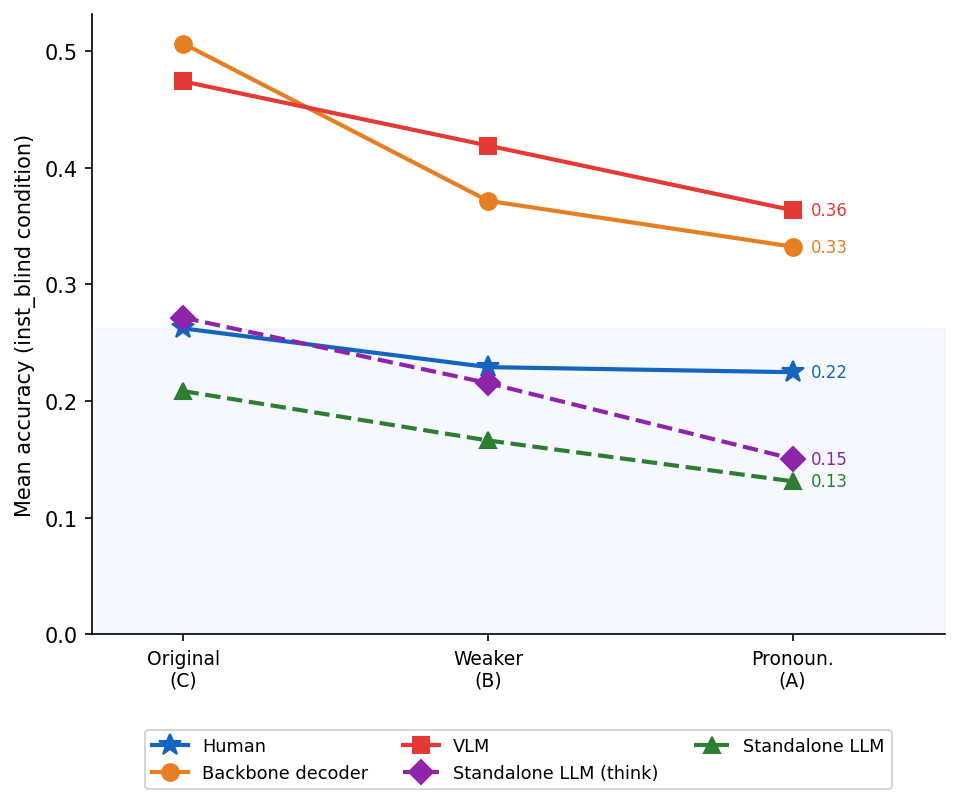
\includegraphics[width=\columnwidth]{accuracy_variants/inst_blind_vABC_groups_7b}
\caption{Control-variant degradation curves across Original~(C)
$\rightarrow$ Weaker~(B) $\rightarrow$ Pronominalized~(A) for the matched-size
7B--8B architecture comparison on the human-study subset ($q=113$, $h=40$)
under the instructed blind condition. Model groups lose accuracy more sharply
than humans as entity anchors are removed, confirming that blind success relies
heavily on entity-specific priors.}
\label{fig:degradation}
\end{figure}

Figure~\ref{fig:degradation} reveals the core finding: as entity-specific
lexical content is progressively removed---from the original question (C) to a
hypernym-weakened variant (B) to a fully pronominalized form (A)---model
accuracy drops substantially for all groups (VLM: $0.455 \to 0.364$,
backbone decoder: $0.506 \to 0.332$), while human accuracy decreases by only
$0.035$ ($0.262 \to 0.227$). The asymmetric degradation confirms that model
accuracy under blind conditions is driven by entity-specific corpus-frequency
priors: removing the entity name (``dog'') for a pronoun (``it'') collapses the
prior signal, whereas humans can reason about the abstract question structure
regardless. The backbone decoder shows the steepest absolute drop
($\Delta = 0.174$), suggesting its blind advantage is particularly reliant on
entity-specific n-gram co-occurrence rather than general syntactic patterns.
Fine-grained per-entity-type degradation curves are in the Appendix.

\begin{figure}[t]
\centering

\includegraphics[width=\columnwidth]{agreement_variants/inst_blind_vABC_sbert_lineplot_q88_h40}
\caption{Human--model SBERT agreement across control variants
  (Original~C $\rightarrow$ Weaker~B $\rightarrow$ Pronominalized~A) on the
  free-text human-comparison subset ($q=88$, $h=39$).
  All model groups lose alignment as entity anchors are removed, mirroring
  the accuracy degradation in Figure~\ref{fig:degradation}. The human--human
  ceiling (dashed) drops only slightly, confirming that the degradation is
  model-specific. Full results for all metrics (chrF, ROUGE-1, BERTScore,
  SimCSE, Jaccard, exact match) are in the supplementary heatmaps.}
\label{fig:agreement_variant}
\end{figure}

\subsection{Instruction-Gated Hallucination}
\label{sec:gated}

A key question is whether models' blind answers reflect a readily available
prior that is always active, or a latent prior that requires explicit
permission to express. We investigate this by comparing model outputs between
the \textbf{Blind} and \textbf{Blind+Inst} conditions.

We classify model outputs in the blind condition as: \textit{hard-abstained}
(explicit refusal: ``I cannot answer'', ``no image''); \textit{soft-abstained}
(hedging outputs: ``nothing'', ``none'', ``unanswerable'', ``nowhere'');
\textit{hallucinated\_correct} (specific answer matching GT); or
\textit{hallucinated\_wrong} (specific answer not matching GT).
Hard abstentions are near-zero across all models (0.0--0.3\%), consistent
with the baked-in ``Answer using a single word'' instruction suppressing
explicit refusals. The real signal is \textit{soft abstention}: 11--19\%
of blind outputs are hedging responses, varying by model family.

\begin{figure}[t]
\centering

\includegraphics[width=\columnwidth]{instruction_effect/merged_abstention_vC_q113}
\caption{Response behavior under Blind and Blind+Inst for variant~C on the
human-study subset. The instruction primarily reduces abstention and converts
hedged outputs into committed answers rather than improving grounding. This
shift is strongest for VLMs and standalone LLMs, while backbone decoders are
comparatively stable.}
\label{fig:gated}
\end{figure}

Figure~\ref{fig:gated} shows the \emph{soft abstention collapse rate}: the
fraction of soft-abstained blind responses that convert to specific answers
under the Blind+Inst instruction. This rate varies dramatically:

\begin{center}
\small
\begin{tabular}{lcc}
\toprule
\textbf{Model} & \textbf{Soft-abs (blind)} & \textbf{Collapse rate} \\
\midrule
Qwen3-VL-8B & 12.9\% & 71.9\% \\
LLaVA v1.6-Mistral & 15.8\% & 51.9\% \\
LLaVA v1.6-Vicuna & 11.3\% & 28.3\% \\
LLaVA v1.5 & 18.7\% & 17.1\% \\
\bottomrule
\end{tabular}
\end{center}

We interpret this spectrum as measuring the degree to which prior activation
is \textit{instruction-gated}. Qwen3-VL, a highly instruction-tuned model,
largely suppresses its prior under blind conditions but rapidly activates it
when given permission. LLaVA v1.5, by contrast, hallucinates
\textit{unconditionally}: it produces specific answers whether or not
instructed to, and shows almost no response to the permission instruction.
This distinction is mechanistically important: instruction-gated models have
a functioning ``uncertainty'' signal that instruction can override, while
unconditional models lack this gate entirely.

Additionally, 33.6\% of all answers (not just soft-abstentions) change between
blind and blind+inst conditions for Qwen3-VL-8B---a large behavioral shift
driven by a single sentence. The yes/no distribution shifts from 70\% ``no''
in blind to 55\% ``yes'' in blind+inst, consistent with the instruction
activating a ``plausible scenario exists'' prior that overrides the default
epistemic null.

\subsection{Confidence Calibration}
\label{sec:confidence}

Confidence analysis reveals that blind hallucinations are produced with high
token-level confidence rather than cautious uncertainty. The instruction does
not merely change \emph{which} answer is produced; it shifts mass away from
abstentions and toward committed outputs that remain highly confident at the
token level.

\begin{figure}[t]
\centering
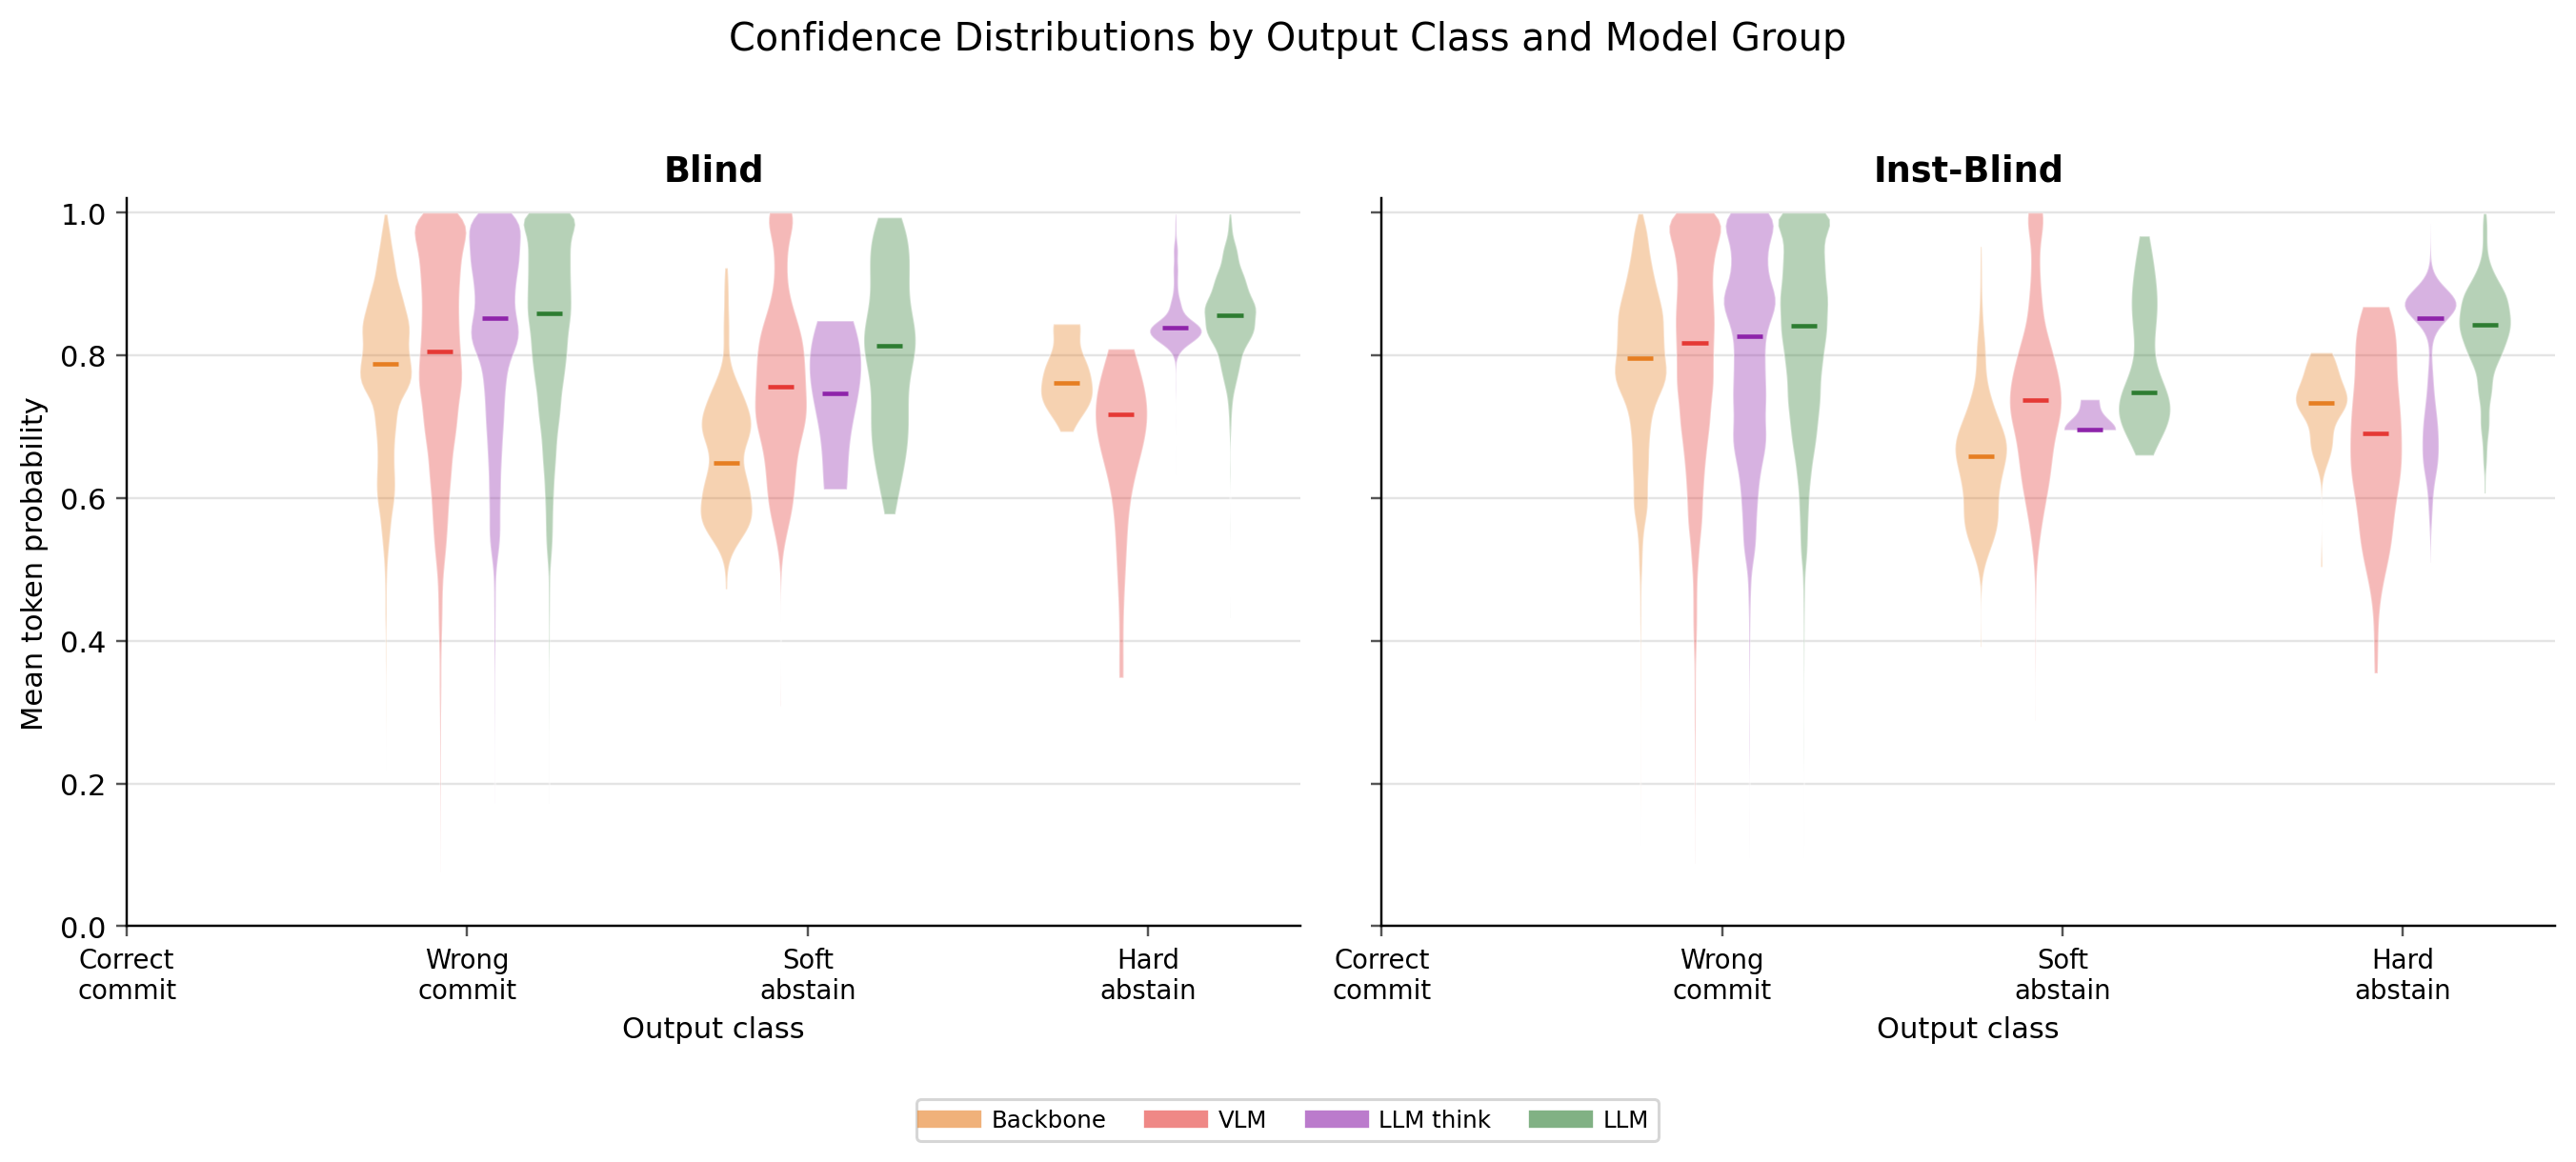
\includegraphics[width=\columnwidth]{confidence_dist/output_class_shift_q113_h40}
\caption{Distribution of mean token probability by output class under Blind and
Blind+Inst on the human-study subset ($q=113$, $h=40$), shown as violin
distributions by model group. Wrong committed answers remain in a high-
confidence regime, while abstentions occupy a lower-confidence regime. The
instruction shifts outputs from abstention toward confident commitment rather
than toward calibrated uncertainty.}
\label{fig:confidence_shift}
\end{figure}

Soft-abstained outputs occupy a lower-confidence regime than committed answers,
confirming that hedging responses reflect genuine uncertainty. However, the
gap is modest, and the baseline level of confidence even for wrong committed
answers remains high. The primary failure is therefore not underconfidence but
confident hallucination.

Quantifying this overconfidence with Expected Calibration Error and testing the
corpus-frequency correlation \citep{mccoy2024embers} directly are reserved for
future work.

% ─────────────────────────────────────────────────────────────────────────────
\section{Human-Model Alignment}
\label{sec:alignment}

The central result of this section is architectural: when models answer VQA
questions without images, the group closest to human blind responses is the
VLM backbone decoder, not the full VLM. VLM backbone decoders (the language
backbone extracted without the vision encoder) reach the highest human-model
SBERT similarity ($0.501$), within $0.067$ of the human-human ceiling
($0.568$). Full VLMs are lower ($0.480$), while standalone LLMs span a much
wider range.

The key point is therefore architectural rather than purely descriptive: the
model component that best recovers human blind priors is the language backbone
exposed in the decoder-only setting, not the full vision-language stack. The
entity-type analysis that follows explains where this alignment is strongest.

\subsection{Humans as a Reference for Prior Structure}
\label{sec:human_ref}

Human participants answering without images still rely on world knowledge and
linguistic priors, but they are not shaped by the same corpus-frequency
objective that drives pretrained LLMs. This makes human blind behavior a
reference for what \emph{linguistically natural} uncertainty looks like---as
opposed to what the training distribution would predict.

The contrast is sharpest in answer distributions (Figure~\ref{fig:dist}).
For yes/no questions, VLMs default to ``no'' 62\% of the time, while humans
lean toward ``yes'' 67\%---the opposite direction. For count questions, 70\%
of VLM answers are ``0'' while humans produce a distributed count distribution
(modal answer: 2, followed by 1 and 3). This reversal is not a calibration gap
in the same direction; it indicates that the model prior is qualitatively
different from the human prior for these question types.

\subsection{Which Models Are Most Human-Like?}
\label{sec:model_similarity}

Not all model families align equally with human blind behavior. We compare four
groups---VLMs, VLM backbone decoders (the same language backbone without the
vision encoder), standalone LLMs, and thinking-mode LLMs---using both
difficulty correlation and pairwise answer similarity. The main interpretive
question is whether the model component that best matches humans is the visual
stack, the language backbone, or the instruction-tuning regime layered on top.

\paragraph{Pairwise answer similarity.}
We compute pairwise SBERT cosine similarity \citep{wang2020minilm} between all
answer pairs (human-human, human-model, model-model) across the 374 free-text
control questions. Human-human agreement provides the ceiling:
$\overline{\text{SBERT}}_{\text{HH}} = 0.568$.
VLM backbone decoders reach $0.501$---closest to the human ceiling---while
full VLMs score $0.480$, standalone LLMs $0.398$, and thinking-mode LLMs $0.426$.
The gap between backbone decoders and full VLMs ($\Delta = 0.021$) is
consistent across lexical metrics (exact match, chrF) and semantic metrics
(SimCSE and BERTScore), indicating that removing the vision encoder does \emph{not} hurt
human alignment and may even improve it by reducing the model's reliance on
spurious visual features.

\paragraph{Difficulty correlation by model group.}
Pearson correlation between per-question human accuracy $h(q)$ and per-model
accuracy further separates the groups. Under blind conditions, VLMs correlate at
$r = 0.50$--$0.62$; backbone decoders at $r = 0.58$--$0.68$; standalone LLMs
at $r = 0.35$--$0.55$. The Blind+Inst condition consistently raises correlations
by up to $\Delta r = +0.10$ for VLMs, narrowing the gap to the human reference.
This pattern is consistent with the instruction-gated hallucination result
(Section~\ref{sec:gated}): receiving the ``imagine the scene'' instruction pushes
models to activate the same distributional priors that drive human performance on
these questions.

\paragraph{Effect of scale on human alignment.}
Within-family scale trends are comparatively weak: human--model SBERT
alignment does not improve monotonically with parameter count, indicating that
alignment with human blind priors is determined more by architecture and
instruction-tuning regime than by raw scale. Detailed scale plots are provided
in the Appendix.

\paragraph{Inter-rater structure.}
Supplementary inter-rater heatmaps show that human participants cluster
separately from all model groups, confirming a qualitative difference in
reasoning strategy rather than a mere accuracy gap. Backbone decoders sit
closest to the human cluster, standalone LLMs furthest. Krippendorff's
$\alpha$ decreases when any model is added to the human rater pool (from
$0.554$ to $0.535$--$0.543$), but the decrease is smallest for backbone
decoders, reinforcing that the language backbone is the primary driver of
human-like prior structure in VLMs.

\subsection{Shared vs.\ Divergent Priors by Entity Type}
\label{sec:prior_types}

Not all questions trigger the same degree of human-model prior alignment.
The entity taxonomy introduced in Section~\ref{sec:control} provides the
analytical structure: entity groups form coherent semantic categories in the
question set, making entity type a principled grouping dimension for alignment
analysis.

We measure \textbf{difficulty correlation}---Pearson $r$ between per-question
human accuracy $h(q)$ and VLM accuracy---within each of the 9 entity types
across 113 questions. Figure~\ref{fig:hm_alignment} shows the distribution of
questions by entity type (left) and the resulting correlations (right).

\begin{figure*}[t]
\centering
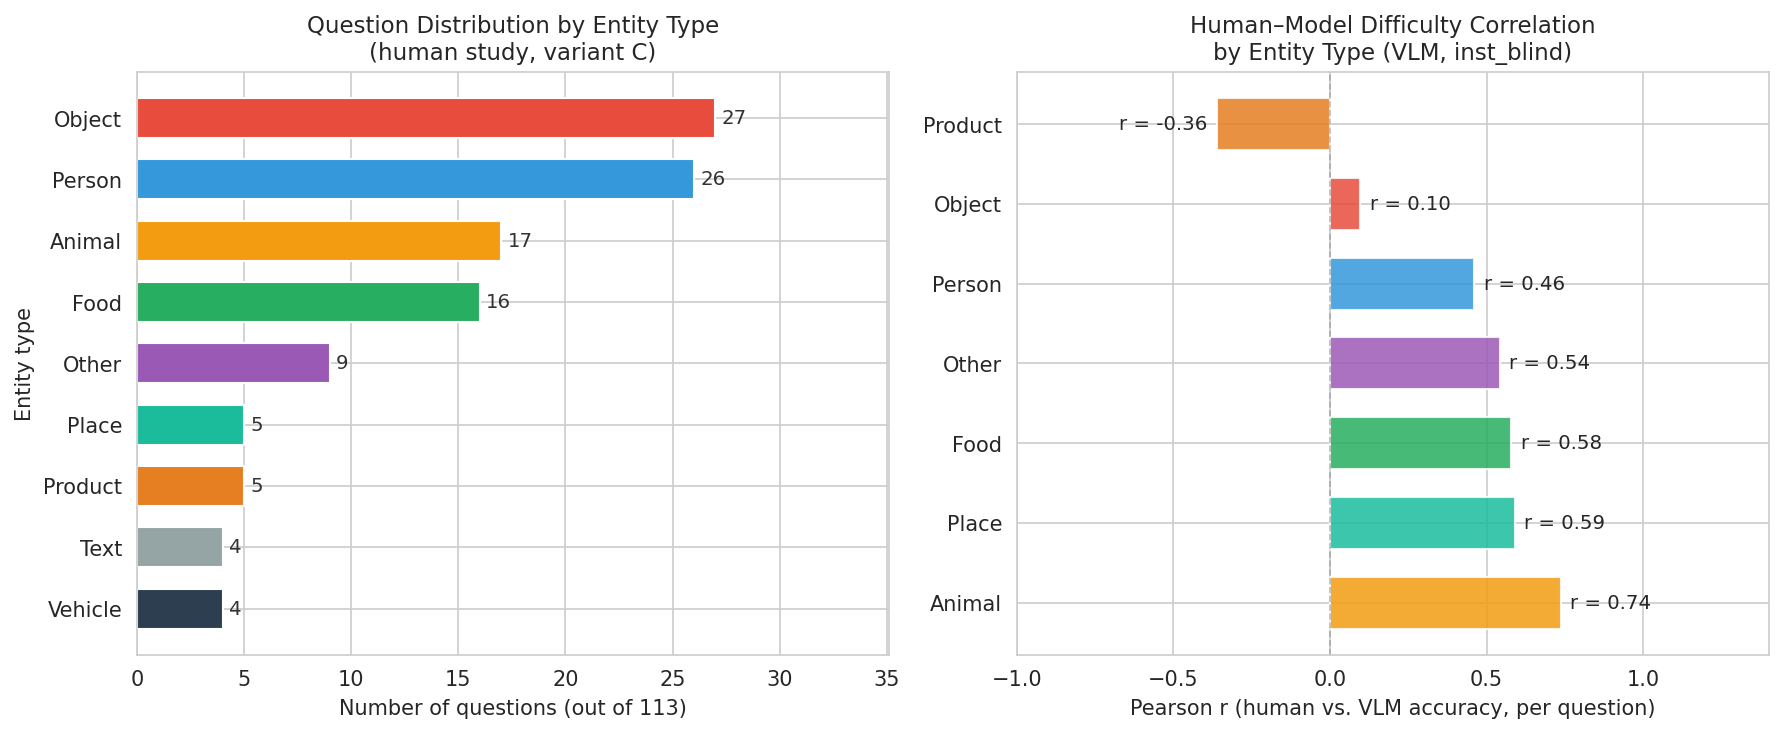
\includegraphics[width=\textwidth]{entity_analysis/fig_hm_alignment_m348}
\caption{\textbf{Left:} distribution of 113 study questions by entity type.
  Object and person dominate; place, product, text, and vehicle have small
  samples ($n \leq 5$).
  \textbf{Right:} Pearson $r$ between per-question human accuracy and VLM
  accuracy (inst\_blind, variant C) within each entity type.
  Animal ($r=0.90$) and place ($r=0.91$) questions show near-perfect
  human--model alignment; food and person show moderate alignment
  ($r=0.77$, $0.64$). Object questions show weak alignment ($r=0.13$),
  while product questions are anti-aligned ($r=-0.48$), indicating that
  human and model difficulty patterns diverge for product-related queries.}
\label{fig:hm_alignment}
\end{figure*}

Three alignment regimes emerge:

\paragraph{Strong alignment (animal, place).}
Animal and place questions show near-perfect human--model difficulty
correlation ($r = 0.90$, $0.91$). Both humans and models exploit the
same entity-specific corpus frequencies for these categories---questions
about animals or locations tend to have predictable answers that align
with statistical regularities in training data.

\paragraph{Moderate alignment (food, person, other).}
Food ($r = 0.77$) and person ($r = 0.64$) entities show moderate alignment.
Models capture the broad easy/hard structure of human difficulty but diverge
on ambiguous cases, particularly for person questions where identity and
contextual knowledge interact.

\paragraph{Divergence (object, product).}
Object questions show weak alignment ($r = 0.13$), reflecting the
high diversity of object categories that span many prior strengths.
Product questions are anti-aligned ($r = -0.48$): when humans succeed
on product queries, models tend to fail, likely because product-specific
prior knowledge is sparser in model training data than in human experience.

The per-question scatter and quadrant-style diagnostics are provided in the
Appendix. They show that shared priors are strongest when both parties are
either similarly uncertain or similarly knowledgeable, while count and product
questions drive many of the strongest divergences.

\subsection{Human-Model Divergence in Answer Patterns}

We measure human-model alignment using two complementary metrics.
First, we compute \textbf{Pearson difficulty correlation}: for each question
$q$, we compute the human group accuracy $h(q)$ (proportion of 36 participants
correct) and correlate it with per-model accuracy.
We prefer Pearson over Spearman here because the relationship is approximately
linear (max $|r - \rho| = 0.026$ across all conditions), and operating on
proportions avoids the information loss from rank conversion on binary data.
Second, we compute \textbf{Krippendorff's $\alpha$} (nominal scale, binary
correctness) to measure within-group and cross-group reliability.

Human difficulty estimates are highly reliable: $\text{ICC}(2,36) = 0.963$
across 36 raters, justifying use of $h(q)$ as a stable difficulty signal.
Within-group human reliability is $\alpha_{\text{human}} = 0.554$ (moderate,
appropriate for a genuinely ambiguous task without visual input).

Pretrained VLMs show moderate correlation with human difficulty under blind
conditions (Pearson $r = 0.50$--$0.62$ depending on model), confirming that
human and model difficulty patterns partially overlap---both exploit linguistic
priors to some extent. However, adding any model to the human rater pool
\emph{decreases} $\alpha$ (from 0.554 to 0.535--0.543), confirming that models
are structurally less consistent with the human group than humans are with each
other.

In the current analysis, Blind+Inst often yields slightly higher
human-difficulty correlations than Blind alone for several model families.
This pattern is consistent with the soft-abstention-collapse result in
Section~\ref{sec:gated}, but it should be treated as provisional until the
human comparison conditions are fully matched across settings.

Appendix heatmaps quantify the same structural separation from a different
angle: human-human similarity exceeds all cross-group scores, humans form a
distinct cluster, and backbone decoders sit closest to that cluster. The
pattern is consistent across lexical and semantic metrics.

Semantic similarity analysis reinforces this finding: model answers have
higher embedding similarity to ground truth (mean 65.8 vs.\ human 64.2)
despite being generated without visual evidence, and the human similarity
distribution has a longer left tail (more diverse wrong answers), consistent
with exploratory reasoning rather than prior retrieval.

% ─────────────────────────────────────────────────────────────────────────────
\section{Discussion}

\paragraph{The instruction-gated spectrum as an architectural insight.}
The dramatic variation in soft-abstention collapse rates (17\% for LLaVA v1.5
vs.\ 72\% for Qwen3-VL) suggests that instruction-following capability plays
a role in prior activation that goes beyond accuracy. Instruction-tuned models
have learned to gate prior expression behind contextual permission signals, while
models with weaker instruction following leak priors unconditionally. This is
not simply a capability difference---LLaVA v1.5 is competitive on standard VQA
accuracy---but a behavioral difference in how priors are accessed.

\paragraph{Implications for benchmark design.}
Our results suggest that any VQA benchmark can be partially solved by
linguistic priors alone, and that the magnitude of this effect varies
predictably with question type, answer distribution, and entity specificity.
We propose that blind VQA evaluation should become a standard diagnostic for
new VQA benchmarks: a high blind accuracy ($>$40\%) is at least a warning sign
that the benchmark may over-index on knowledge-accessible question types.

\paragraph{Limitations.}
Our human study involves 36 participants recruited from university communities
in a single language (Korean/English), limiting cultural and demographic
generalizability. Model evaluation uses greedy decoding (temperature 0), which
may underestimate answer diversity and overestimate confidence. The control
variant GPT extraction uses a best-effort seed (seed is advisory in the
Responses API) and results may vary slightly across runs. Human data was
collected under the Blind+Inst condition only, so direct comparisons with model
blind (no instruction) behavior rely on the assumption that the instruction
has a comparable normalizing effect on humans and models---an assumption our
instruction-gated analysis partially supports but does not fully validate.
A direct corpus-frequency correlation---testing whether per-question blind accuracy
predicts answer frequency in the VQA v2 training distribution---would strengthen the
mechanistic account \citep{mccoy2024embers} and is deferred to future work.

% ─────────────────────────────────────────────────────────────────────────────
\section{Conclusion}

We present a human-calibrated diagnostic study of linguistic prior exploitation
in Vision-Language Models. Analogous to hypothesis-only baselines in NLI, blind
VQA reveals that VLMs produce characteristic answer distribution biases shaped
by training-corpus frequencies---and that these biases are only partially shared
with human blind reasoners. We introduce control question variants to probe how
lexical cues drive prior activation, and use token-confidence analysis to
expose the severe overconfidence that accompanies blind hallucination. The
instruction-gated spectrum reveals a behavioral axis across model families that
is invisible to accuracy-only evaluation.

The central finding of the human alignment study is that prior sharing is
question-type-specific. Yes/no and action questions show near-complete
human-model overlap (Jaccard $\approx 0.93$), while count and grounded-reference
questions are anti-aligned (difficulty $r = -0.39$). The model zero-bias and
no-bias are not linguistic priors in any human sense---they are model-specific
failure modes. At the architecture level, VLM backbone decoders
(language backbone without vision encoder) achieve near-human pairwise answer
similarity ($0.501$ vs.\ human $0.568$), and their yes/no distribution reverts
to human-like rates when the vision encoder is removed, confirming that the
no-bias is a VLM artifact rather than a corpus-frequency prior. These findings argue that diagnosing prior exploitation requires attending to both
the language backbone and the vision--language integration layer separately.

% ─────────────────────────────────────────────────────────────────────────────
\bibliography{paper}

% ─────────────────────────────────────────────────────────────────────────────
\appendix

\section{Human Study Protocol}
\label{app:human}

A total of 36 participants (15 men and 21 women; age range: 18--34 years) were
included in the study. Participants were recruited via online student community
forums at universities. All procedures were conducted under an IRB-approved
protocol and adhered to the principles of the Declaration of Helsinki. Informed
consent was obtained from all participants prior to participation.

Each participant completed 113 VQA-style questions. Participants were
compensated at a rate of 10,000 KRW per hour, consistent with standard
compensation for similar annotation tasks.

For VQA, participants were instructed to provide free-form answers that were as
concise as possible. Responses could be given in either Korean or English and
were translated and processed using the same answer normalization and aggregation
strategy described in Appendix~\ref{app:aggregation}.

\section{Answer Aggregation}
\label{app:aggregation}

We cluster semantically equivalent answers (e.g., ``3'' and ``three'') into
canonical forms using GPT-4o mini \citep{openai2025gpt4o}. The prompt instructs
the model to group synonymous responses, select the most concise canonical form,
and return results in structured JSON. Human responses are then aggregated into
a confidence-weighted distribution over canonical answers, where each answer's
weight is the sum of confidence scores from all annotators selecting that answer,
normalized to sum to 1:
\begin{equation}
H(a_k^*) = \frac{\sum_{i:\phi(a_i)=a_k^*} c_i}{\sum_i c_i}
\end{equation}
where $c_i$ is participant $i$'s Likert confidence (normalized to $[0,1]$),
$\phi$ maps raw answers to canonical answers, and $K$ is the number of
canonical answer clusters.

\section{Control Question Extraction Prompt}
\label{app:ctl}

Control variants are extracted using GPT-4.1-mini-2025-04-14 (temperature 0,
seed 42) with strict JSON schema mode for reproducibility.
The system prompt instructs the model to generate all four variants in a single
API call per batch of 50 questions. The schema enforces:
\texttt{\{deictic\_removed, object\_removed, weaker\_object, pronominalized\}}
as required string fields, with \texttt{additionalProperties: false}.
For pronominalized, the prompt specifies grammar-aware substitution rules to
ensure natural pronominalization (``What color is it?'' not ``What color is
the object?'').

\section{Blind VQA Accuracy Summary}
\label{app:accuracy}

\begin{table*}[h]
\centering
\caption{Zero-shot blind VQA performance of humans and models.
Y/N = yes/no accuracy; Num = numerical; Other = open-ended (Accuracy/Similarity).
Bold: best; underline: second best.}
\label{tab:main}
\small
\begin{tabular}{lll rrrr}
\toprule
\textbf{Model} & \textbf{LLM} & \textbf{Size} & Y/N & Num & Other & Avg \\
\midrule
Humans (N=36) & -- & -- & 66.6 & 13.8 & 13.0/45.5 & 39.0 \\
\midrule
\multicolumn{7}{l}{\textit{LLM Baseline (text-only)}} \\
\multirow{2}{*}{Qwen3} & \multirow{2}{*}{Qwen3} & 4B
    & 54.9 & 19.0 & 24.7/55.2 & 38.8 \\
 & & 8B & 50.3 & 17.1 & 22.1/53.2 & 35.3 \\
\midrule
\multicolumn{7}{l}{\textit{VLM (blind)}} \\
\multirow{3}{*}{Qwen3-VL} & \multirow{3}{*}{Qwen3} & 2B
    & 71.8 & 17.1 & 23.8/55.5 & 46.4 \\
 & & 4B & 71.5 & 19.0 & \underline{28.9}/\underline{56.4} & \underline{48.0} \\
 & & 8B & 71.5 & 21.9 & 27.0/54.9 & \textbf{48.0} \\
\midrule
LLaVA v1.5 & Vicuna & 7B & 70.3 & 17.1 & 19.4/48.4 & 43.8 \\
LLaVA v1.6 & Mistral & 7B & 69.6 & 20.0 & 27.0/55.0 & 47.0 \\
LLaVA v1.6 & Vicuna & 7B & 74.4 & 20.0 & 27.2/56.2 & \underline{49.4} \\
\bottomrule
\end{tabular}
\end{table*}

\section{Blind Awareness Instruction}
\label{app:inst}

After the original prompt and the blank image, models in the Blind+Inst
condition receive: \textit{``Note: No images are provided. For each question,
imagine an appropriate image exists and answer based on the most common or
universal scenario.''}

Table~\ref{tab:inst_effect} shows accuracy comparison between Blind and
Blind+Inst conditions on VQA. The instruction usually changes accuracy by only
a few points, confirming that it does not reliably improve performance even when
it substantially changes answer behavior.

\begin{table}[h]
\centering
\caption{VQA accuracy comparison with and without blind instruction.
$\Delta_{\text{inst}} = \text{Blind}_{\text{inst}} - \text{Blind}$.}
\label{tab:inst_effect}
\small
\begin{tabular}{l rrr}
\toprule
\textbf{Model} & GT & Blind & $\Delta$ \\
\midrule
InternVL3.5-1B & 80.5 & 43.6 & 0.2 \\
InternVL3.5-2B & 82.1 & 45.5 & -0.2 \\
InternVL3.5-4B & 83.0 & 45.0 & 2.2 \\
InternVL3.5-8B & 86.9 & 47.1 & -1.7 \\
\midrule
Qwen3-VL-2B & 83.0 & 45.0 & 0.7 \\
Qwen3-VL-4B & 85.9 & 45.5 & 1.9 \\
Qwen3-VL-8B & 89.4 & 44.3 & 3.1 \\
\bottomrule
\end{tabular}
\end{table}

% ─────────────────────────────────────────────────────────────────────────────
\section{Supplementary Per-Question and Scale Diagnostics}
\label{app:diagnostics}

The main text emphasizes group-level results. This appendix collects the
per-question and scale-sensitive views that support the same claims but are too
dense for the main paper.

\begin{figure}[h]
\centering
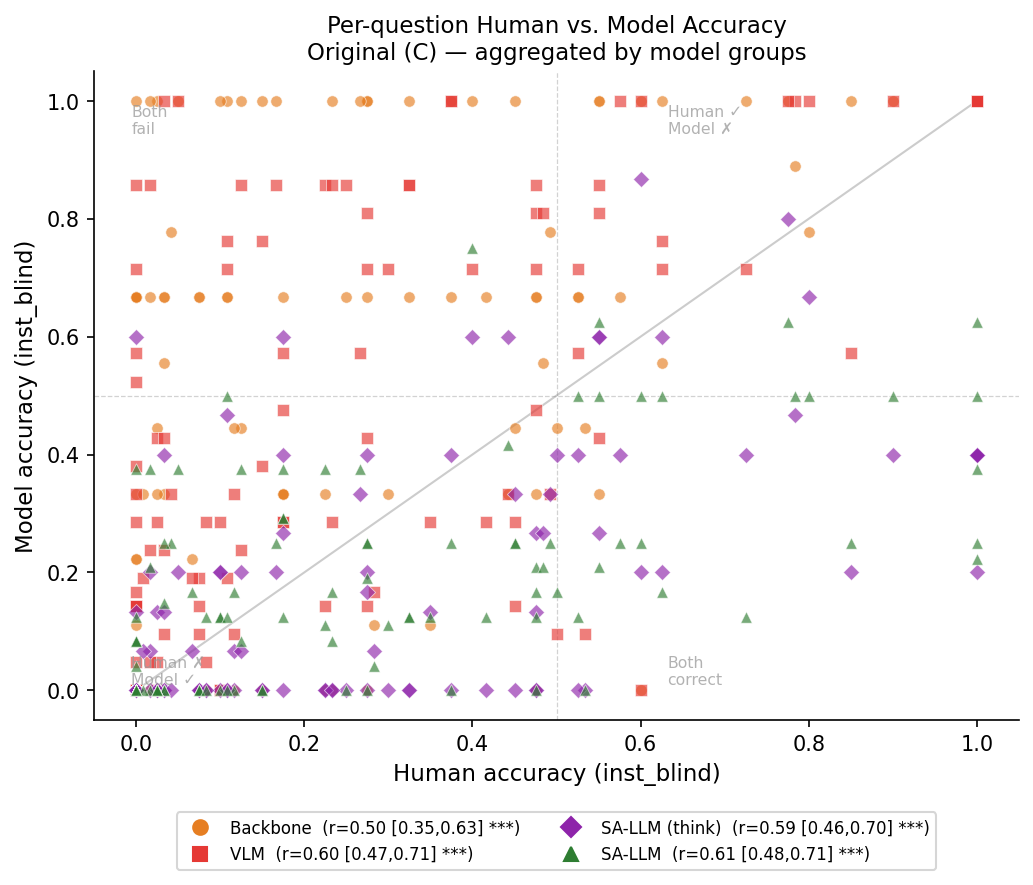
\includegraphics[width=\columnwidth]{accuracy_scatter/inst_blind_vC_groups_q113_h40}
\caption{Per-question human accuracy versus model accuracy on the instructed
blind human-study subset ($q=113$, $h=40$), faceted by model group. This raw
scatter underlies the aggregated control-variant trends in
Figure~\ref{fig:degradation}.}
\label{fig:app_acc_scatter}
\end{figure}

\begin{figure}[h]
\centering
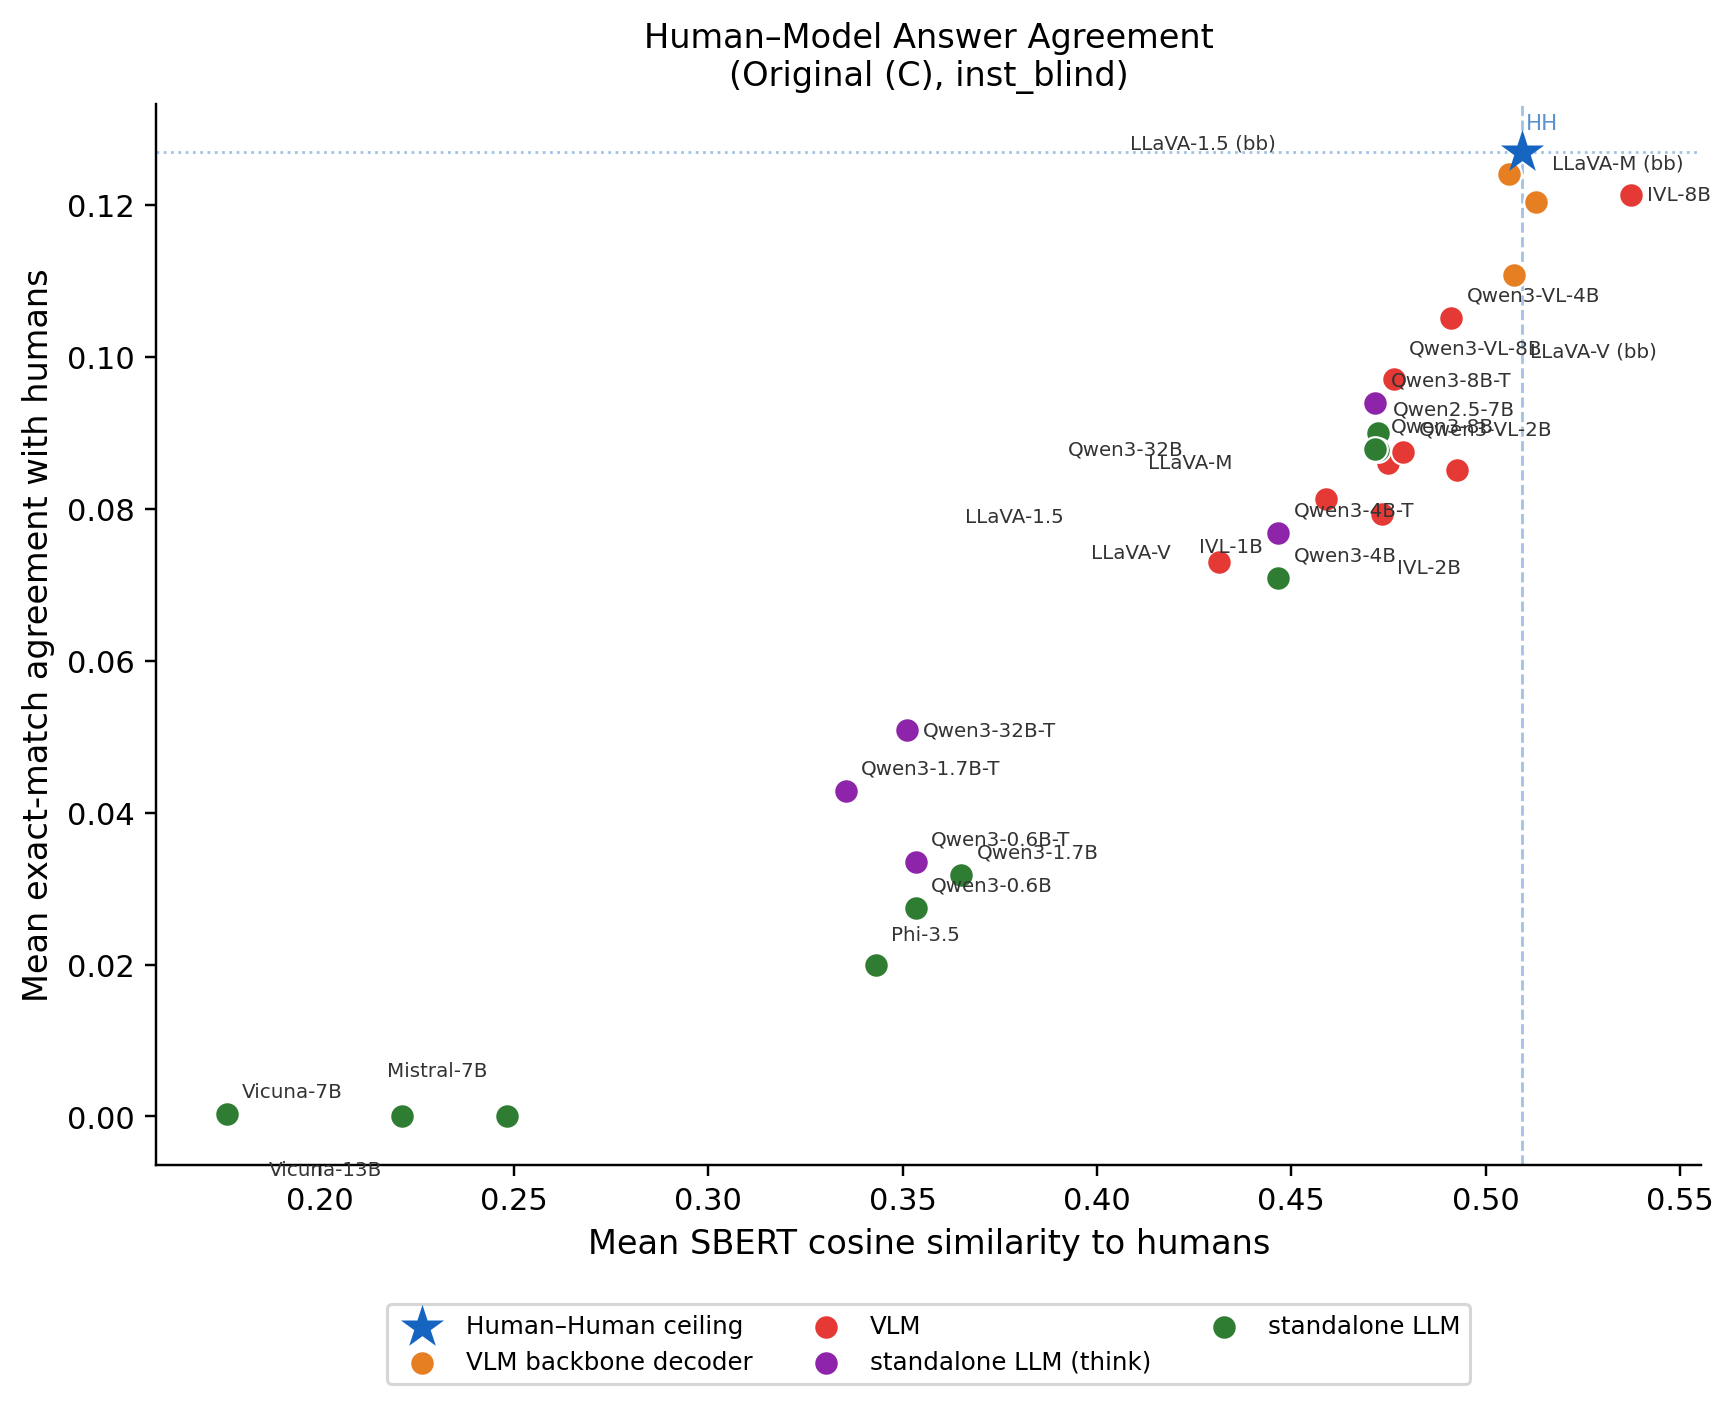
\includegraphics[width=\columnwidth]{agreement_scatter/inst_blind_vC_sbert_exact_models_q88_h40}
\caption{Per-model human--model agreement on the free-text subset
($q=88$, $h=39$). X-axis: mean SBERT similarity to human answers. Y-axis:
mean exact-match agreement. This figure makes the same group separation as the
main text visible at model granularity.}
\label{fig:app_agreement_scatter}
\end{figure}

\begin{figure}[h]
\centering

\includegraphics[width=\columnwidth]{agreement_scale/inst_blind_groups_sbert_vC_q113_h40_yesno}
\caption{Human--model SBERT agreement versus model scale by model group on the
inst\_blind variant-C human-comparison subset. Scale effects are weaker than
the architectural differences emphasized in the main text.}
\label{fig:app_scale}
\end{figure}

% ─────────────────────────────────────────────────────────────────────────────
\section{Answer Distribution by Model Group (Notebook 13)}
\label{app:dist13}

Figure~\ref{fig:dist_appendix} repeats the blind-condition answer-distribution
comparison from the main text. A fuller notebook-driven breakdown by all model
groups and both Blind / Blind+Inst conditions remains part of the analysis
pipeline, but the current main paper claims only require the VLM-versus-human
contrast shown here.

\begin{figure}[h]
\centering

\includegraphics[width=\columnwidth]{answer_dist/inst_blind_vC_yn_q26_h40}

\includegraphics[width=\columnwidth]{answer_dist/inst_blind_vC_number_q26_h40}
\caption{Answer-distribution biases under the instructed blind condition across
all model groups. Top: yes/no answers. Bottom: count answers. The descriptive
patterns remain structured, but matched-size and model-group comparisons are
best interpreted as robustness checks rather than as the main architectural
evidence.}
\label{fig:dist_appendix}
\end{figure}

% ─────────────────────────────────────────────────────────────────────────────
\section{Agreement by Control Variant — All Metrics}
\label{app:agreement_variant}

Figures~\ref{fig:av_simcse}--\ref{fig:av_exact} extend Figure~\ref{fig:agreement_variant}
from \S\ref{sec:degradation} to all remaining agreement metrics.
Each lineplot shows mean human--model agreement per model group across the three
control variants (Original\,C $\to$ Weaker\,B $\to$ Pronominalized\,A),
with the human--human ceiling (dashed blue) as reference.
Each heatmap summarises the same data as a group$\times$variant grid.
The consistent downward trend across all metrics confirms that entity
removal reduces human--model alignment independent of the metric used.

\begin{figure}[h]
\centering

\includegraphics[width=\columnwidth]{agreement_variants/inst_blind_vABC_simcse_lineplot_q88_h40}
\caption{Human--model SimCSE cosine agreement across control variants (by model group).}
\label{fig:av_simcse}
\end{figure}

\begin{figure}[h]
\centering

\includegraphics[width=\columnwidth]{agreement_variants/inst_blind_vABC_simcse_heatmap_q88_h40}
\caption{SimCSE agreement heatmap (group $\times$ variant, HM pairs).}
\label{fig:av_simcse_heat}
\end{figure}

\begin{figure}[h]
\centering

\includegraphics[width=\columnwidth]{agreement_variants/inst_blind_vABC_bertscore_lineplot_q88_h40}
\caption{Human--model BERTScore F1 across control variants.}
\label{fig:av_bertscore}
\end{figure}

\begin{figure}[h]
\centering

\includegraphics[width=\columnwidth]{agreement_variants/inst_blind_vABC_bertscore_heatmap_q88_h40}
\caption{BERTScore F1 agreement heatmap (group $\times$ variant, HM pairs).}
\label{fig:av_bertscore_heat}
\end{figure}

\begin{figure}[h]
\centering

\includegraphics[width=\columnwidth]{agreement_variants/inst_blind_vABC_chrf_lineplot_q88_h40}
\caption{Human--model chrF across control variants.}
\label{fig:av_chrf}
\end{figure}

\begin{figure}[h]
\centering

\includegraphics[width=\columnwidth]{agreement_variants/inst_blind_vABC_chrf_heatmap_q88_h40}
\caption{chrF agreement heatmap (group $\times$ variant, HM pairs).}
\label{fig:av_chrf_heat}
\end{figure}

\begin{figure}[h]
\centering

\includegraphics[width=\columnwidth]{agreement_variants/inst_blind_vABC_rouge1_lineplot_q88_h40}
\caption{Human--model ROUGE-1 across control variants.}
\label{fig:av_rouge1}
\end{figure}

\begin{figure}[h]
\centering

\includegraphics[width=\columnwidth]{agreement_variants/inst_blind_vABC_rouge1_heatmap_q88_h40}
\caption{ROUGE-1 agreement heatmap (group $\times$ variant, HM pairs).}
\label{fig:av_rouge1_heat}
\end{figure}

\begin{figure}[h]
\centering

\includegraphics[width=\columnwidth]{agreement_variants/inst_blind_vABC_jaccard_lineplot_q88_h40}
\caption{Human--model token Jaccard across control variants.}
\label{fig:av_jaccard}
\end{figure}

\begin{figure}[h]
\centering

\includegraphics[width=\columnwidth]{agreement_variants/inst_blind_vABC_jaccard_heatmap_q88_h40}
\caption{Token Jaccard agreement heatmap (group $\times$ variant, HM pairs).}
\label{fig:av_jaccard_heat}
\end{figure}

\begin{figure}[h]
\centering

\includegraphics[width=\columnwidth]{agreement_variants/inst_blind_vABC_exact_lineplot_q88_h40}
\caption{Human--model exact-match rate across control variants.}
\label{fig:av_exact}
\end{figure}

\begin{figure}[h]
\centering

\includegraphics[width=\columnwidth]{agreement_variants/inst_blind_vABC_exact_heatmap_q88_h40}
\caption{Exact-match heatmap (group $\times$ variant, HM pairs).}
\label{fig:av_exact_heat}
\end{figure}

% ─────────────────────────────────────────────────────────────────────────────
\section{SBERT Agreement by Control Variant — Group Heatmaps}
\label{app:sbert_variant_heat}

Figure~\ref{fig:av_sbert_heat} provides the heatmap counterpart to the SBERT
lineplot shown in Figure~\ref{fig:agreement_variant} (\S\ref{sec:degradation}).
Rows correspond to model groups and the human--human baseline; columns to the
three control variants.

\begin{figure}[h]
\centering

\includegraphics[width=\columnwidth]{agreement_variants/inst_blind_vABC_sbert_heatmap_q88_h40}
\caption{SBERT cosine agreement heatmap (group $\times$ variant, HM pairs).
Colour scale shared with Figure~\ref{fig:agreement_variant}.}
\label{fig:av_sbert_heat}
\end{figure}

% ─────────────────────────────────────────────────────────────────────────────
\section{Inter-rater Agreement Heatmaps — All Metrics}
\label{app:interrater_all}

Figures~\ref{fig:cm_sbert_groups}--\ref{fig:cm_exact_full} summarize the
inter-rater agreement structure for variant\,C under the inst\_blind
condition.
In each figure, the top panel shows group-mean agreement and the bottom panel
shows the full per-rater matrix (36 humans + all model groups).
The block structure is consistent across metrics: humans cluster tightly
together, backbone decoders agree more with humans than full VLMs do, and
standalone LLMs (especially thinking-mode variants) occupy a distinct region.

\begin{figure}[h]
\centering

\includegraphics[width=\columnwidth]{agreement_heatmaps/vC_sbert_groups}
\caption{SBERT cosine inter-rater agreement --- group-mean matrix (variant C).}
\label{fig:cm_sbert_groups}
\end{figure}

\begin{figure}[h]
\centering

\includegraphics[width=\columnwidth]{agreement_heatmaps/vC_sbert_all}
\caption{SBERT cosine inter-rater agreement --- full per-rater matrix (variant C).}
\label{fig:cm_sbert_full}
\end{figure}

\begin{figure}[h]
\centering

\includegraphics[width=\columnwidth]{agreement_heatmaps/vC_simcse_groups}
\caption{SimCSE cosine inter-rater agreement --- group-mean matrix (variant C).}
\label{fig:cm_simcse}
\end{figure}

\begin{figure}[h]
\centering

\includegraphics[width=\columnwidth]{agreement_heatmaps/vC_simcse_all}
\caption{SimCSE cosine inter-rater agreement --- full per-rater matrix (variant C).}
\label{fig:cm_simcse_full}
\end{figure}

\begin{figure}[h]
\centering

\includegraphics[width=\columnwidth]{agreement_heatmaps/vC_bertscore_groups}
\caption{BERTScore F1 inter-rater agreement --- group-mean matrix (variant C).}
\label{fig:cm_bertscore}
\end{figure}

\begin{figure}[h]
\centering

\includegraphics[width=\columnwidth]{agreement_heatmaps/vC_bertscore_all}
\caption{BERTScore F1 inter-rater agreement --- full per-rater matrix (variant C).}
\label{fig:cm_bertscore_full}
\end{figure}

\begin{figure}[h]
\centering

\includegraphics[width=\columnwidth]{agreement_heatmaps/vC_chrf_groups}
\caption{chrF inter-rater agreement --- group-mean matrix (variant C).}
\label{fig:cm_chrf}
\end{figure}

\begin{figure}[h]
\centering

\includegraphics[width=\columnwidth]{agreement_heatmaps/vC_chrf_all}
\caption{chrF inter-rater agreement --- full per-rater matrix (variant C).}
\label{fig:cm_chrf_full}
\end{figure}

\begin{figure}[h]
\centering

\includegraphics[width=\columnwidth]{agreement_heatmaps/vC_rouge1_groups}
\caption{ROUGE-1 F1 inter-rater agreement --- group-mean matrix (variant C).}
\label{fig:cm_rouge1}
\end{figure}

\begin{figure}[h]
\centering

\includegraphics[width=\columnwidth]{agreement_heatmaps/vC_rouge1_all}
\caption{ROUGE-1 F1 inter-rater agreement --- full per-rater matrix (variant C).}
\label{fig:cm_rouge1_full}
\end{figure}

\begin{figure}[h]
\centering

\includegraphics[width=\columnwidth]{agreement_heatmaps/vC_jaccard_groups}
\caption{Token Jaccard inter-rater agreement --- group-mean matrix (variant C).}
\label{fig:cm_jaccard}
\end{figure}

\begin{figure}[h]
\centering

\includegraphics[width=\columnwidth]{agreement_heatmaps/vC_jaccard_all}
\caption{Token Jaccard inter-rater agreement --- full per-rater matrix (variant C).}
\label{fig:cm_jaccard_full}
\end{figure}

\begin{figure}[h]
\centering

\includegraphics[width=\columnwidth]{agreement_heatmaps/vC_exact_groups}
\caption{Exact-match inter-rater agreement --- group-mean matrix (variant C).}
\label{fig:cm_exact}
\end{figure}

\begin{figure}[h]
\centering

\includegraphics[width=\columnwidth]{agreement_heatmaps/vC_exact_all}
\caption{Exact-match inter-rater agreement --- full per-rater matrix (variant C).}
\label{fig:cm_exact_full}
\end{figure}

\end{document}
